\documentclass{standalone}
\usepackage{tikz}
\usepackage{ctex,siunitx}
\usepackage{tkz-euclide}
\usepackage{amsmath}
\usetikzlibrary{patterns, calc}
\usetikzlibrary {decorations.pathmorphing, decorations.pathreplacing, decorations.shapes,}
\begin{document}
\small
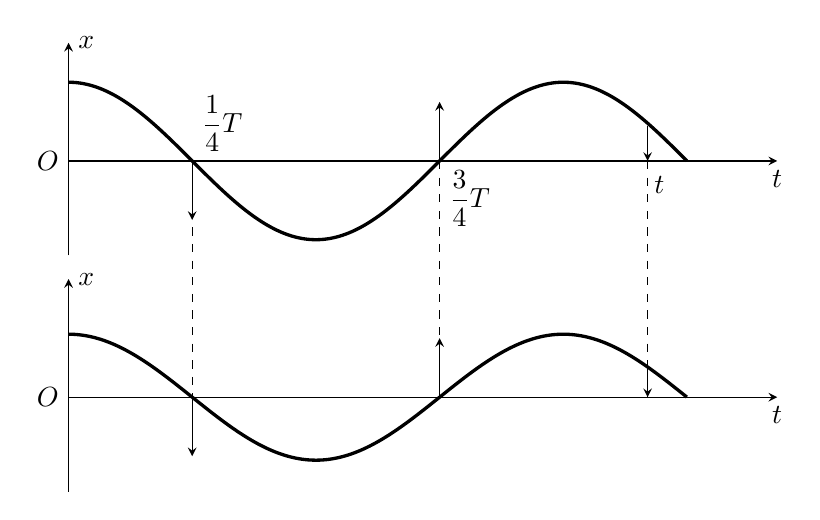
\begin{tikzpicture}[>=stealth, scale=1, domain=0:2.5*pi, samples=200]
  \draw [->](0,0)node [left]{$O$}--(9,0) node [below]{$t$};
  \draw [->](0,-1.2)--(0,1.5) node [right]{$x$};
  \draw [->](0,-3)node [left]{$O$}--(9,-3) node [below]{$t$};
  \draw [->](0,-4.2)--(0,-1.5) node [right]{$x$};
  \draw [very thick]  plot (\x,{cos(\x r)});
  \draw [very thick]  plot (\x,{.8*cos(\x r)-3});
  \draw [dashed](.5*pi, 0) -- (.5*pi, 0-3);  
  \draw [dashed](1.5*pi, 0) -- (1.5*pi, 0-3);     
  \draw [dashed](2.5*pi-.5, 0) -- (2.5*pi-.5, 0-3);     
  \draw [->](.5*pi, 0)node [above right]{$\dfrac{1}{4}T$}--(.5*pi,-.75);
  \draw [->](.5*pi, 0-3)--(.5*pi,-.75-3);
  \draw [->](1.5*pi, 0)node [below right]{$\dfrac{3}{4}T$} -- (1.5*pi, .75);    
  \draw [->](1.5*pi, 0-3) -- (1.5*pi, .75-3);    
  \draw [<-](2.5*pi-.5, 0) -- (2.5*pi-.5, .44);  
  \draw [<-](2.5*pi-.5, 0-3) -- (2.5*pi-.5, .44-3);  
  \node at (2.5*pi-.35, -.3){$t$};
\end{tikzpicture}
\end{document}